\section{Theory}
\subsection{Introduction}
Diodes are non-linear circuit components which only allows the unidirectional flow of current. A diode basically consists of a P-N junction with metallic contacts at the end for application of external voltage. The direction of arrow indicates the conventional direction of current flow, from P-side to N-side.

\begin{figure}[H]
    \centering
    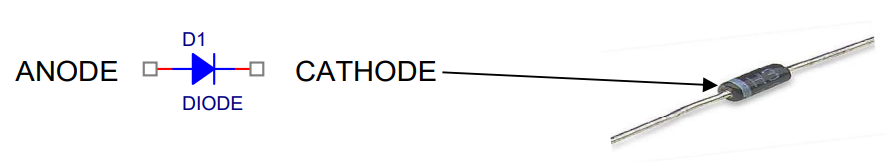
\includegraphics[width=0.8\columnwidth]{images/d1.png}
    \caption{Circuit symbol of a diode and a commercial diode}
\end{figure}

During the formation of the P-N junction, due to the concentration gradient across P, and N-sides, holes diffuse from P-side to N-side and electrons diffuse from N-side to P-side. This gives rise to a \textbf{diffusion current}, and a \textbf{depletion region} is formed at the junction consisting of immobile charges. Due to this, there is a \textbf{barrier potential} across the depletion region.

Theoretical equation for the diode current ($I_D$) is,
\begin{equation}
    I_D = I_s\left[\exp{\frac{V_D}{nV_T}} - 1\right]
\end{equation}

where $V_D$ = voltage drop across the diode, $I_S$ = saturation current, $V_T = k_BT/q$ ($\approx 0.026V$ at $T=300K$) is the thermal voltage, and $n$ is the emission coefficient. The emission coefficient accounts for recombinations of electrons and holes in the depletion region, which tends to decrease the current. For discrete diodes, $n = 2$ and in intergrated circuits, $n=1$.


An \textit{ideal} diode works as a short circuit in forward bias and an open circuit in reverse bias. However, in a real diode, the current faces resistance due to the potential barrier. When the applied potential is more than the potential barrier, the current through the diode increases steeply.

\begin{figure}[H]
     \centering
     \begin{subfigure}[b]{0.35\textwidth}
         \centering
         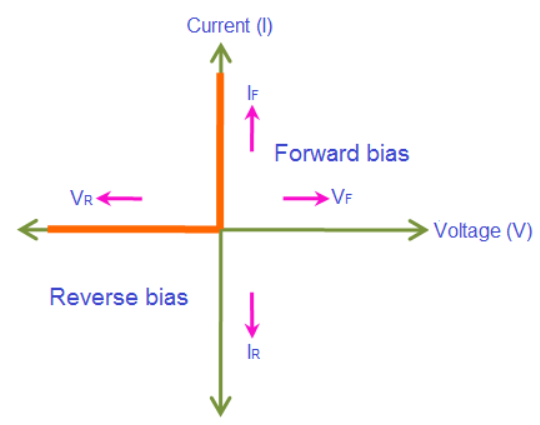
\includegraphics[width=\textwidth]{images/d2.png}
         % \caption{(a)}
     \end{subfigure}
     \hfill
     \begin{subfigure}[b]{0.35\textwidth}
         \centering
         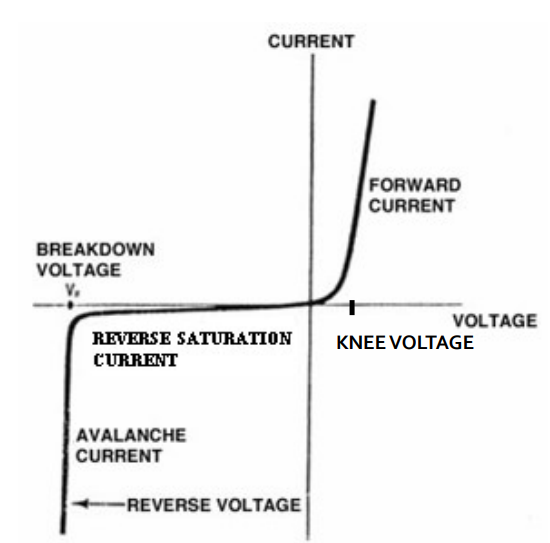
\includegraphics[width=\textwidth]{images/d3.png}
         % \caption{(b)}
     \end{subfigure}
     \hfill
        \caption{I-V characteristics of (a) an ideal diode and (b) a real diode}
\end{figure}

\subsubsection{Biasing a diode}

\begin{enumerate}
    \item \textbf{Forward bias:} When the P-side is connected to the positive and N-side to the negative terminals of the power supply, it reduces the potential barrier. As a result current flows from P to N-type in forward direction. When the applied voltage is more than the barrier potential, the resistance is small (ideally 0) and the current increases rapidly. This point is called the \textit{Knee-point} or \textit{threshold voltage}. This voltage is about 0.3 V Ge-diodes and 0.7 V for Si diodes. 

    \item \textbf{Reverse bias:} Here, the P-side of the junction diode is connected to the negative and N-side is connected to the positive terminal of the power supply. This increases the potential barrier due to which ideally no current should flow. But in practice, the minority carriers can tr, known as the \textit{reverse saturation current}. This current is about 2-20 $\mu$A for Ge diodes and 2-20 nA for Si diodes.
\end{enumerate}

If the reverse bias is made too high, the current through the diode increases abruptly at a certain voltage, known as the \textbf{breakdown voltage}. In conventional (lightly doped) diodes, this is due to collisions of large number of thermally generated electrons in a phenomena called the \textbf{avalanche breakdown}.


\subsection{Zener Diodes}
These are a specific type of diodes with heavily doped PN junctions. The forward characteristic of a zener diode is similar to a normal diode. \textbf{Zener voltage} is the reverse voltage above which there is a controlled breakdown which does not damage the diode. The voltage drop across the diode remains constant at zener voltage no matter how high the reverse bias voltage is.

\begin{figure}[H]
    \centering
    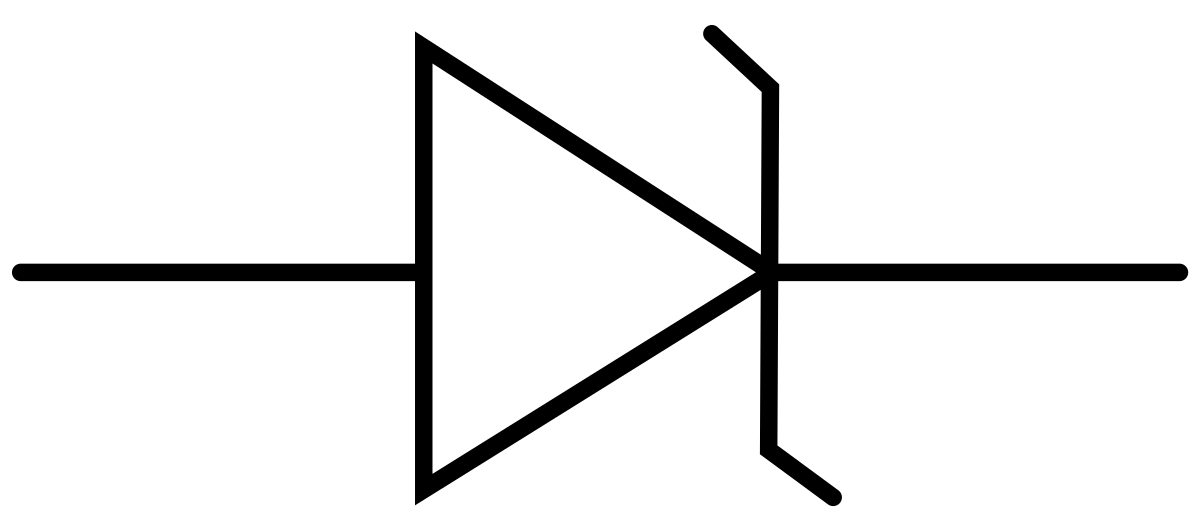
\includegraphics[width=0.2\columnwidth]{images/d4.png}
    \caption{Circuit symbol of a zener diode}
\end{figure}

Since the PN-junction is heavily doped, the depletion layer is narrow for a zener diode. At high reverse voltages, the high electric field created at the narrow depletion region generates a large number of electron hole pairs causing high current to flow. This process is called the \textbf{Zener breakdown}.


\subsection{Static and Dynamic Resistance}
The static or the DC resistance, $R_D$ at any given point is given by inverse of the slope at that point of the I-V characteristic of the diode. The static resistance is higher below the knee voltage
than above the knee voltage.

\begin{equation}
    R_D = \frac{V_D}{I_D}
\end{equation}

Since diode resistance dynamically varies with the input voltage, we define a term dynamic resistance --- $r_D$ --- to measure the resistance at an instantaneous operating point. The dynamic resistance or the AC resistance is defined as the ratio of change in voltage and change in current around the DC operating point.

\begin{equation}
    r_D = \frac{\Delta V_D}{\Delta I_D}
\end{equation}

\begin{figure}[H]
    \centering
    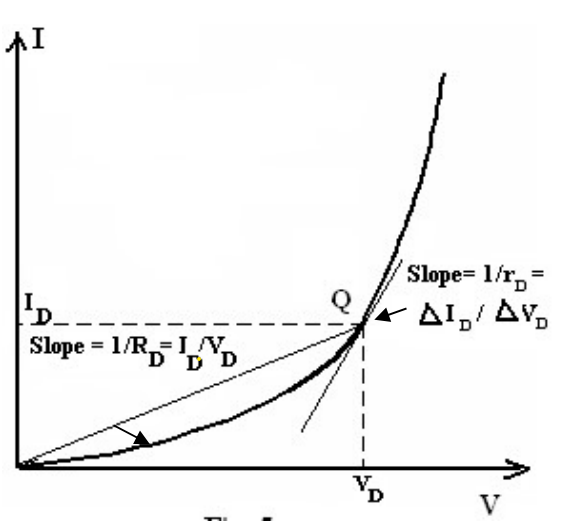
\includegraphics[width=0.6\columnwidth]{images/d5.png}
    \caption{Finding Static and Dynamic Resistance of diode from the I-V plot}
\end{figure}

\subsection{Application}
Diodes have extremely important applications in modern electronics. They are used in communication systems as limiters, clippers, gates, in power supply systems as rectifiers and inverters, voltage multipliers and so on.

Zener diodes in particular are used for voltage regulation as the voltage drop across the diode remains constant over a wide range of voltages. They are also used as surge suppressors to prevent  accidental overloads in circuits.